\documentclass[11pt]{article}
\usepackage[margin=0.8in]{geometry}
\usepackage{amsmath}
\usepackage{amssymb}
\usepackage[hypcap=false]{caption}
\usepackage{capt-of}
\usepackage{graphicx}
\usepackage{tikz-cd}
\usepackage{multicol}
\usepackage{fancyhdr}
\usepackage[table]{xcolor}
\usepackage{titlesec}
\usepackage{tocloft}
\usepackage{microtype}
\usepackage{tabularx}
\usepackage{booktabs}
\usepackage[colorlinks=true]{hyperref}

\definecolor{TOCBlue}{HTML}{1F4E79}
\definecolor{SectionBlue}{HTML}{4F81BD}
\definecolor{techgray}{gray}{0.90}

\hypersetup{
  linkcolor=TOCBlue,
  citecolor=TOCBlue,
  urlcolor=TOCBlue
}

% TOC: show sections only (hide subsections)
\setcounter{tocdepth}{1}

% Make "\*" safe in math mode (used in a few places like $\mathcal{T}^\*$)
\DeclareRobustCommand{\*}{\ast}

% Reduce/suppress minor overfull/underfull \hbox warnings
\setlength{\emergencystretch}{6em}
\hbadness=10000
\hfuzz=25pt
\tolerance=2000
\pretolerance=1000

% TOC styling (blue) + tighter spacing to keep it to one page
\renewcommand{\contentsname}{\textcolor{TOCBlue}{Contents}}
\renewcommand{\cftsecfont}{\color{TOCBlue}}
\renewcommand{\cftsecpagefont}{\color{TOCBlue}}
\setlength{\cftbeforetoctitleskip}{0pt}
\setlength{\cftaftertoctitleskip}{6pt}
\setlength{\cftbeforesecskip}{0pt}

% Section heading color (lighter blue)
\titleformat{\section}{\color{SectionBlue}\normalfont\Large\bfseries}{\thesection}{1em}{}

% Running header
\pagestyle{fancy}
\fancyhf{}
\lhead{Modernizing MISO Deliverability}
\rhead{TP-006}
\cfoot{\thepage}
\renewcommand{\headrulewidth}{0.4pt}
\setlength{\headheight}{13.6pt}
\addtolength{\topmargin}{-1.6pt}


% ---------- TikZ / diagrams ----------
\usepackage{tikz}
\usetikzlibrary{
  arrows.meta,
  positioning,
  calc,
  shapes.geometric,
  shapes.misc,
  fit
}

% ---------- Theorem environments (for formal propositions / claims) ----------
\newtheorem{proposition}{Proposition}
\newtheorem{definition}{Definition}
\newtheorem{remark}{Remark}

% ---------- Core macros ----------
\newcommand{\PRM}{\mathrm{PRM}}
\newcommand{\LOLE}{\mathrm{LOLE}}
\newcommand{\EUE}{\mathrm{EUE}}
\newcommand{\VOLL}{\mathrm{VOLL}}
\newcommand{\ELCC}{\mathrm{ELCC}}
\newcommand{\UCAP}{\mathrm{UCAP}}
\newcommand{\NQC}{\mathrm{NQC}}
\newcommand{\LMP}{\mathrm{LMP}}

% Usable headroom: H = min(A, D)
\newcommand{\Headroom}{H}
\newcommand{\Accred}{A}
\newcommand{\Deliv}{D}

\begin{document}

\title{Modernizing MISO Deliverability: Benchmarking Hybrid Accreditation Against PJM and CAISO}
\author{Prepared by: Justin Candler \& Uriel}
\date{August 22, 2025}

\maketitle

\begin{abstract}
\textbf{Thesis.} Resource adequacy (RA) is an operating headroom promise. Planners size reserve margins
today so operators can supply energy and operating reserves tomorrow. That promise only holds if (i)
resources are accredited to produce when called and (ii) those MW are deliverable to the binding nodes
under security constraints. In MISO, the capability leg (accreditation/ELCC) has advanced faster than
the deliverability leg for co-located portfolios (e.g., solar + storage behind a shared POI, often with
separate ownership). The result is persistent discounting of otherwise reliable portfolios. This paper
formalizes the three margins that matter (SRMC energy, LRMC-capacity, LRMC-wires), compares
PJM/CAISO/ERCOT constructs, and proposes a minimal set of rule changes that would allow MISO
to convert accredited MW into usable headroom without compromising reliability or market discipline.
\end{abstract}

\begingroup
\small
\setlength{\parskip}{0pt}
\tableofcontents
\endgroup
\clearpage

\section{Executive Summary}

\textbf{Rapid takeaways}
\begin{itemize}
  \item RA = tomorrow's operating headroom. Planning reserves are not abstract; they are the expected
  supply of real-time operating reserves and dispatchable energy in the hours that dominate LOLE.
  \item Two legs, one product. Accreditation (can it produce?) $\times$ Deliverability (can we move it?) $\Rightarrow$ usable
  headroom. Either leg missing $\Rightarrow$ ``paper MW''.\footnote{In UEVF terms, ``paper MW'' typically reflects an accreditation quantity (Reliability Module) that is not
paired with the binding network feasibility/rights (Transmission Module). The orthogonality discipline is the
point: if deliverability is not explicitly specified, it is being implicitly assumed. See: \emph{00 - UEVF.pdf}.}
  \item Co-located portfolios are penalized in MISO because deliverability and scheduling constructs at
  the POI are not yet standardized, especially for separate ownership. Portfolio physics exist; portfolio
  rights do not.
  \item Peers are ahead on deliverability rights. PJM binds capacity eligibility to explicit CIRs; CAISO
  ties NQC to deliverability allocations (FCDS/EODS) and provides clean ``hybrid vs. co-located'' registration
  with a SC. ERCOT relies on energy/AS scarcity pricing (ORDC) rather than a capacity construct, so
  deliverability shows up via planning and nodal price risk.
  \item Minimal fixes for MISO. (1) POI-level portfolio deliverability budgets allocable by a Portfolio Operator
  of Record; (2) unified accreditation of configurable hybrids at the POI; (3) a transparent eligibility
  checklist that equals accreditation $\times$ deliverability; (4) performance-linked settlement in LOLE-weighted
  hours; (5) ownership-agnostic scheduling authority and telemetry.
\end{itemize}

\textbf{One graphic worth keeping in mind}

% =========================================================
% TikZ FIGURE — "R → A → D → H" pipeline
% Place this where you currently have “One graphic worth keeping in mind”
% or at the start of Section 2.
% =========================================================

\begin{figure}[ht]
\centering
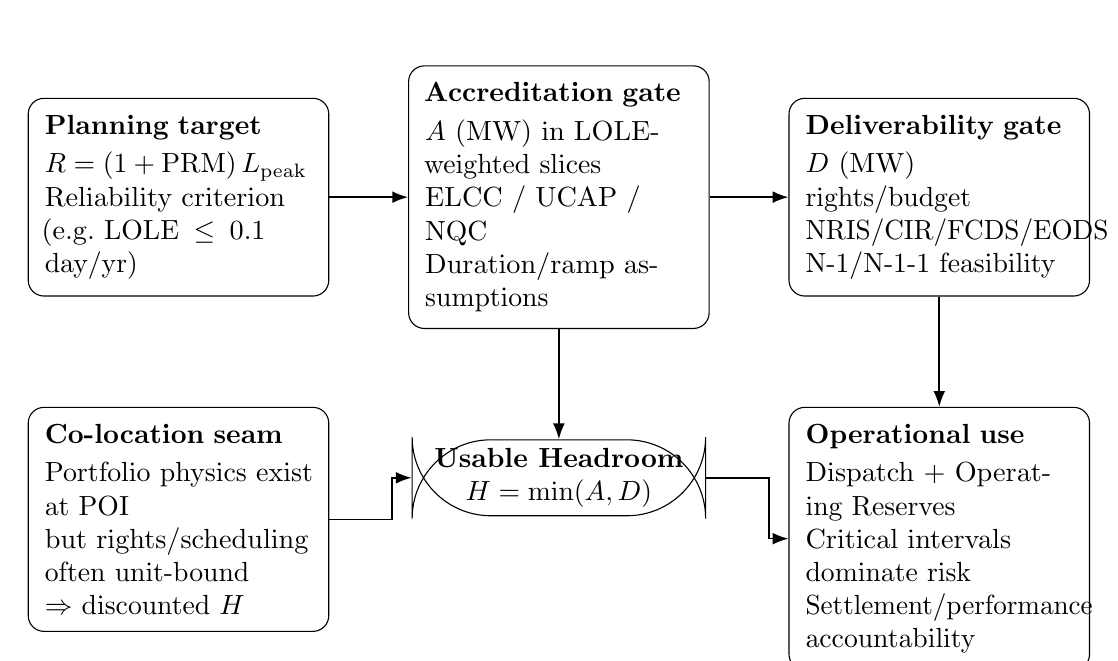
\begin{tikzpicture}[
  node distance=12mm and 10mm,
  box/.style={draw, rounded corners=2mm, align=left, inner sep=6pt, text width=0.28\linewidth},
  pill/.style={draw, rounded corners=10mm, align=center, inner ysep=3pt, inner xsep=8pt},
  arr/.style={-Latex, line width=0.6pt}
]

% Left: planning target
\node[box] (prm) {\textbf{Planning target}\\[2pt]
$R=(1+\PRM)\,L_{\text{peak}}$\\
Reliability criterion (e.g.\ $\LOLE \le 0.1$ day/yr)};

% Accreditation
\node[box, right=of prm] (A) {\textbf{Accreditation gate}\\[2pt]
$\Accred$ (MW) in LOLE-weighted slices\\
ELCC / UCAP / NQC\\
Duration/ramp assumptions};

% Deliverability
\node[box, right=of A] (D) {\textbf{Deliverability gate}\\[2pt]
$\Deliv$ (MW) rights/budget\\
NRIS/CIR/FCDS/EODS\\
N-1/N-1-1 feasibility};

% Usable headroom
\node[pill, below=of A, yshift=-2mm] (H) {\textbf{Usable Headroom}\\
$\Headroom=\min(\Accred,\Deliv)$};

% Operator use
\node[box, below=of D, yshift=-2mm] (ops) {\textbf{Operational use}\\[2pt]
Dispatch + Operating Reserves\\
Critical intervals dominate risk\\
Settlement/performance accountability};

% Arrows
\draw[arr] (prm) -- (A);
\draw[arr] (A) -- (D);
\draw[arr] (A.south) -- (H.north);
\draw[arr] (D.south) -- (ops.north);
\draw[arr] (H.east) -- ++(8mm,0) |- (ops.west);

% Annotation: co-location seam
\node[box, below=of prm, yshift=-2mm] (seam) {\textbf{Co-location seam}\\[2pt]
Portfolio physics exist at POI\\
but rights/scheduling often unit-bound\\
$\Rightarrow$ discounted $\Headroom$};

\draw[arr] (seam.east) -- ++(8mm,0) |- (H.west);

\end{tikzpicture}
\caption{From planning reserves to usable headroom: accreditation and deliverability are distinct gates. The operational object is $\Headroom=\min(\Accred,\Deliv)$, not nameplate MW.}
\label{fig:headroom-pipeline}
\end{figure}
Missing either side yields ``paper MW'' that cannot reliably appear in real time.

Conceptual product: accredited and deliverable MW become the dispatcher's usable headroom.

% =========================================================
% REWRITE: Sections 2–6 (drop-in replacement)
% Goal: tighten formalism (min vs product), add PORR pro forma,
% and add steelman hypotheses (H1–H3) without bloating length.
% =========================================================

\section{Resource Adequacy as Tomorrow's Operating Headroom}
\subsection{From planning reserve to real-time headroom}
Let $L_{\text{peak}}$ denote forecast peak load and $\text{PRM}$ the planning reserve margin. Planners size a
capacity target
\begin{equation}
R = (1 + \text{PRM})\, L_{\text{peak}},
\end{equation}
to meet a probabilistic reliability criterion (e.g., annual LOLE $\le 0.1$ day). Operationally, however, the
system does not consume $R$ as an abstract scalar. Operators need \emph{deliverable} MW in the specific
intervals that dominate risk (the LOLE-weighted slices). The bridge from planning $R$ to operational
headroom has two distinct gates:

\begin{itemize}
  \item \textbf{Accreditation (capability):} what MW can be expected to produce when called in reliability-critical
  intervals (ELCC/UCAP/NQC-like constructs).
  \item \textbf{Deliverability (network \& rights):} what MW can be injected and moved to binding load under
  security constraints, consistent with the commercial rights structure (NRIS/CIR/FCDS/EODS, etc.).
\end{itemize}

\subsection{A tighter definition of ``usable headroom''}
The paper's thesis can be stated without ambiguity by separating (i) accredited capability from (ii) deliverable
rights/budgets and (iii) the operational quantity the dispatcher can actually rely upon.

Define:
\begin{itemize}
  \item $A$ = accredited capability (MW) for a resource (or portfolio) in the relevant reliability slices.
  \item $D$ = deliverability budget/rights (MW) available to that same resource (or portfolio) to move power
  to load under security constraints.
\end{itemize}

Then \textbf{usable headroom} is bounded by both legs:
\begin{equation}
H \;=\; \min(A,\;D).
\end{equation}

This is the operational object that matters: regardless of how large $A$ is, the dispatcher cannot count more
than $D$; likewise, regardless of how large $D$ is, the system cannot count more than $A$.

\vspace{0.5em}
\noindent\textbf{Relationship to the ``two-leg'' product intuition.} If it is useful to express deliverability as a factor, define
$\delta \in [0,1]$ as an effective deliverability fraction relative to a chosen reference $P$ (e.g., POI export
limit or nameplate), where $D=\delta P$. If accreditation is also expressed as a factor $\eta$ via $A=\eta P$, then
\begin{equation}
H \;=\; \min(\eta P,\;\delta P) \;=\; P\cdot \min(\eta,\;\delta),
\end{equation}
which preserves the ``two legs'' intuition while remaining dimensionally consistent.

\subsection{Three margins that matter: SRMC energy, LRMC capacity, LRMC wires}
\textbf{(a) SRMC energy.} At node $i$ and time $t$, the short-run marginal price is
\begin{equation}
\text{LMP}_{i,t} = \lambda_t + \sum_k \mu_{k,t}\, \text{PTDF}_{i,k} + \text{loss}_{i,t},
\end{equation}
where $\lambda_t$ is the system marginal energy cost, $\mu_{k,t}$ the congestion shadow prices, and
$\text{PTDF}_{i,k}$ the shift factors. This governs dispatch and operating behavior at the margin.

\textbf{(b) LRMC capacity.} To maintain reliability under growth, a peak-coincident increment $\Delta d$ requires
roughly $(1+\text{PRM})\,\Delta d$ of \emph{accredited} capacity. The cost is technology- and location-dependent
because accreditation is LOLE-slice specific (ELCC is not nameplate).

\textbf{(c) LRMC wires.} Security constraints (thermal/voltage/stability) make deliverability discrete and locational.
Large additions at a bus or POI can change binding N-1 or N-1-1 constraints, triggering lumpy upgrades.
This is a \emph{separate} long-run margin from LRMC capacity.

\subsection{Why co-located portfolios expose the seam}
Co-located solar + storage behind one POI can increase effective headroom in net-peak hours by shifting
energy intra-day and reducing curtailment. The physics is portfolio-like. But if $D$ is granted and enforced
as a \emph{unit-bound} right rather than a \emph{POI/portfolio budget}, then the market cannot reliably translate
portfolio physics into $H=\min(A,D)$ at the times that dominate LOLE. That is the seam: portfolio value exists
in dispatch; portfolio rights often do not exist in eligibility, scheduling authority, and auditable performance
accountability.

\subsection{Relationship to UEVF/ASCDE: why this paper isolates a single missing interface}
This paper should be read as a targeted sub-result within the Unified Energy Valuation Framework (UEVF).
UEVF decomposes project value into orthogonal modules, including a \emph{Reliability Module} (adequacy and
accreditation via ELCC/UCAP/NQC) and a \emph{Transmission Module} (the cost and feasibility of delivering that
capability to binding load under security constraints).\footnote{UEVF defines ASCDE as an all-in, system-adjusted
cost per delivered MWh that starts from base costs (LCOE-like) and then adds/subtracts non-overlapping module
adders/credits, including reliability and transmission effects. The module structure is designed to be largely
orthogonal to minimize double counting and to force explicit attribution of constraints. See: \emph{00 - UEVF.pdf}.}

TP-006 isolates the \emph{interface operator} between these modules: converting accredited capability into
\emph{usable operating headroom} requires explicit deliverability rights at the POI that can be allocated in a way
that matches portfolio physics. When rights remain unit-bound while physics is portfolio-bound, the market
produces ``paper MW''—accredited in planning constructs but not reliably producible at the constrained nodes.

\begin{figure}[h]
\centering
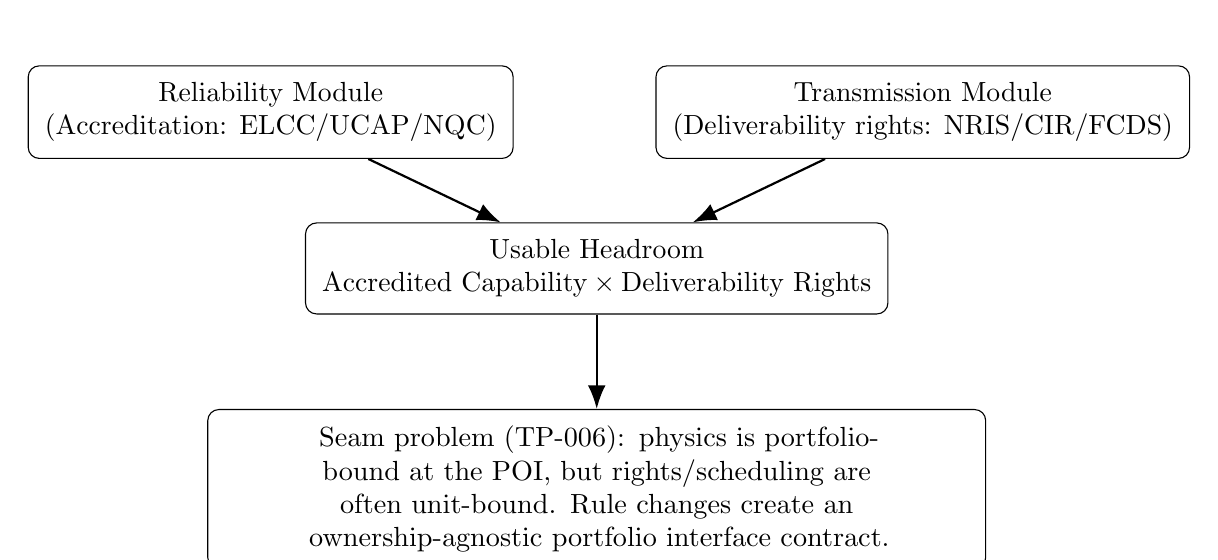
\begin{tikzpicture}[
  box/.style={draw, rounded corners, align=center, inner sep=6pt},
  arrow/.style={-{Latex[length=3mm]}, thick}
]
\node[box] (rel) {Reliability Module\\(Accreditation: ELCC/UCAP/NQC)};
\node[box, right=18mm of rel] (tx) {Transmission Module\\(Deliverability rights: NRIS/CIR/FCDS)};
\node[box, below=14mm of $(rel)!0.5!(tx)$] (head) {Usable Headroom\\$\text{Accredited Capability} \times \text{Deliverability Rights}$};

\draw[arrow] (rel) -- (head);
\draw[arrow] (tx) -- (head);

\node[box, below=12mm of head, text width=0.78\linewidth] (seam)
{Seam problem (TP-006): physics is portfolio-bound at the POI, but rights/scheduling are often unit-bound.
Rule changes create an ownership-agnostic portfolio interface contract.};

\draw[arrow] (head) -- (seam);
\end{tikzpicture}
\caption{TP-006 as a UEVF interface problem: converting accredited MW into deliverable operating headroom.}
\label{fig:uevf-interface}
\end{figure}

\section{Definitions, Notation, and Stylized Example}

\subsection{Key definitions}
\begin{itemize}
  \item \textbf{Accreditation (ELCC/UCAP/NQC):} an estimate of callable MW in reliability-critical intervals,
  generally time-slice dependent.
  \item \textbf{Deliverability:} the ability/right to inject and move MW to load under security constraints (N-1/N-1-1),
  consistent with the ISO's deliverability construct (NRIS/CIR/FCDS/EODS or analog).
  \item \textbf{Co-located:} two or more resources sharing a POI (may be separately owned).
  \item \textbf{Hybrid:} resources registered and modeled as a single entity with unified control and telemetry.
  \item \textbf{Usable headroom:} $H=\min(A,D)$ in the relevant reliability slices.
\end{itemize}

\subsection{Stylized case (used throughout)}
Consider a 300 MW PV plant and a 200 MW/800 MWh battery behind the same POI at 230 kV. Peak-hour
PV curtailment recurs due to a binding 345/230 kV bank or downstream thermal constraint. Portfolio control
could (i) absorb PV surplus into storage, (ii) shift discharge into net-peak hours, and (iii) provide a more
reliable headroom contribution in LOLE-weighted slices. Yet if deliverability $D$ is allocated as unit-bound
rights (and dispatch authority/telemetry is fragmented across owners), the market may only recognize
fragments of the portfolio's potential $A$ as operationally countable $H$.

\section{Cross-ISO Constructs for Accreditation and Deliverability}

This section compares how peers translate accredited capability into deliverable, enforceable RA headroom. The key question is: \emph{how does each ISO define and police $D$ (deliverability) for purposes of counting or monetizing $H=\min(A,D)$?}

\vspace{1em}

% Define a custom column type 'L' that is a flexible X column but Left-Aligned (Ragged Right)
\newcolumntype{L}{>{\raggedright\arraybackslash}X}

\begin{table}[htbp]
\centering
\small
\renewcommand{\arraystretch}{1.4} % Increases row height for readability
\rowcolors{2}{white}{techgray!40} % Alternating row colors (requires [table]{xcolor})

\caption{Scorecard: Accreditation, Deliverability Gating, and POI Portfolio Support}
\label{tab:iso_scorecard}

\begin{tabularx}{\linewidth}{@{} l L L L L @{}}
\toprule
\textbf{ISO} & \textbf{Accreditation} & \textbf{Deliverability Gating for RA} & \textbf{Co-located Ownership \& Scheduling at POI} & \textbf{Maturity} \\
\midrule

\textbf{PJM} & 
ELCC for variable; storage rules by duration & 
Capacity eligibility binds to CIR quantity; deliverability tested & 
Combined/separate registration with allocable CIRs; SC-mediated scheduling & 
High \\

\textbf{MISO} & 
Evolving ELCC/UCAP (ZRCs); storage rules in flight & 
NRIS deliverability required; portfolio allocation not standardized & 
Separate ownership/dispatch rights unresolved; eligibility haircuts common & 
Medium--Low \\

\textbf{CAISO} & 
NQC via ELCC for solar/wind/storage/hybrids & 
Deliverability allocations (FCDS/EODS) gate NQC countability & 
Clear hybrid vs. co-located constructs; SC manages portfolio within allocations & 
Medium--High \\

\textbf{ERCOT} & 
No capacity market; contributions show via energy/AS & 
No RA deliverability gate; constraints monetize through LMP/ORDC risk & 
Co-located registration supported; economics via LMP/AS rather than RA & 
Medium \newline \scriptsize{(Different Paradigm)} \\

\bottomrule
\end{tabularx}
\end{table}

\vspace{0.5em}

\noindent\textbf{Interpretation.} PJM and CAISO most explicitly bind eligibility to deliverability rights. ERCOT monetizes deliverability mainly through energy and ancillary service risk rather than a capacity eligibility gate. MISO is most exposed to the co-location seam because accredited capability can exist without a standardized, portfolio-aware deliverability budget and scheduling authority at the POI.

\newpage

\section{Gap Analysis for MISO}

\subsection{Symptoms}
\begin{itemize}
  \item \textbf{Accredited MW without a portfolio-aware $D$.} Projects can receive accreditation on $A$ yet face
  reduced countability or monetization because deliverability $D$ is not recognized or enforceable at the POI
  portfolio level.
  \item \textbf{Ownership penalty.} Separate legal owners behind one POI face unclear dispatch authority, telemetry,
  and performance accountability, reducing bid confidence and leading to de facto discounts.
  \item \textbf{Curtailment lock-in.} Storage that could reduce local PV curtailment is stranded when $D$ is enforced
  as a unit-bound right rather than a POI portfolio budget with auditable intra-interval reallocation.
\end{itemize}

\subsection{Causal mechanisms (rights, eligibility, governance)}
\textbf{1) Rights mismatch.} Physics rewards portfolios; rights are granted to units. Without a POI-level deliverability
budget, reallocation within the POI does not reliably create countable headroom $H$.

\textbf{2) Eligibility coupling.} RA countability is effectively $H=\min(A,D)$ in the relevant slices. A shortfall on either
leg forces discounts regardless of the portfolio's theoretical complementarity.

\textbf{3) Governance friction.} Absent a standardized Portfolio Operator of Record with enforceable authority and
telemetry, separate owners cannot credibly coordinate charging/dispatch to satisfy LOLE-weighted call hours.

\subsection{Steelman alternatives: why co-located portfolios clear at a discount (H1--H3)}
To keep the argument decision-grade (not advocacy-grade), it is useful to state competing hypotheses for
observed discounts and define what evidence would shift beliefs.

\begin{itemize}
  \item \textbf{H1 (Rights mismatch is binding).} The discount is primarily institutional: $D$ is defined and enforced at
  the unit level (or is ambiguous at the POI), so portfolio physics cannot be converted into countable $H$.
  \item \textbf{H2 (Performance risk is binding).} The discount is rational risk pricing: multi-party control, telemetry,
  SOC management, and coordination failures make realized availability in LOLE-weighted slices uncertain,
  so buyers derate even if rights could be defined.
  \item \textbf{H3 (Settlement design is binding).} The discount persists because settlement does not sufficiently
  reward performance in LOLE-critical intervals, so market participants price co-located portfolios as low-value
  even when they could be high-value with the right incentives.
\end{itemize}

\noindent\textbf{What would change the conclusion.} Evidence that single-owner co-located portfolios still clear at the
same discount would push weight away from H1 toward H3; repeated underperformance in named LOLE-weighted
intervals despite clean rights would push weight toward H2.

\section{Proposed Rule Changes (Minimal Set)}

The goal is not to ``favor hybrids.'' The goal is to define an auditable, reliability-safe mechanism that converts
accredited capability into usable headroom: $H=\min(A,D)$, with $D$ defined at the POI portfolio level where the
physics actually occurs.

\subsection{1) POI Portfolio Deliverability Budgets}
Create a metered, allocable deliverability budget at each POI. A designated Portfolio Operator of Record
(PORR; typically the Scheduling Coordinator or a pro forma equivalent) can assign $D$ across units intra-interval,
subject to telemetry, audit, and constraint envelopes. Rights are technology-neutral and ownership-agnostic:
what matters is \emph{control} and \emph{accountability}, not common ownership.

\subsection{2) Unified Accreditation of Configurable Portfolios}
Compute accreditation $A$ on the modeled portfolio with binding POI constraints, rather than as a simple sum of
unit-level ELCC. Publish capacity-configuration curves (e.g., duration vs. accredited MW) by LRZ and POI type,
including de-rates where POI constraints bind in reliability slices.

\subsection{3) Transparent Eligibility Checklist: eligibility is $H=\min(A,D)$}
Make RA eligibility an explicit function of accreditation and deliverability with a public checklist: telemetry
granularity, SOC reporting (if storage), ramp guarantees, outage coordination, POI limit observance, and
performance test procedures. The checklist should make clear which requirements govern $A$, which govern $D$,
and which govern settlement/performance.

\subsection{4) Performance-Linked Settlement in LOLE-Weighted Intervals}
Settle a defined slice of RA credits on availability in LOLE-weighted critical intervals. Portfolios that reliably
produce $H$ in those slices earn the premium; those that miss are derated. Start small (e.g., 10\%) to avoid
excessive revenue volatility while establishing discipline and data.

\subsection{5) Ownership-Agnostic Scheduling Authority and Telemetry}
Authorize the PORR to optimize charging, curtailment sharing, and emergency response under a standard pro
forma arrangement, without requiring common ownership. The mechanism must make telemetry and performance
accountability \emph{portfolio-native} even when assets are separately owned.

\subsection{Minimum viable PORR pro forma (to prevent gaming)}
\noindent A POI portfolio framework fails if it cannot answer: \emph{who is accountable, what is observable, and what is
conserved?} The PORR construct should be the minimum viable governance layer.

\begin{itemize}
  \item \textbf{Control:} PORR has demonstrable authority to dispatch/charge/curtail within the POI limits.
  \item \textbf{Observability:} POI metering + unit telemetry (including SOC where applicable) at a resolution consistent
  with the market interval; data retention for audit.
  \item \textbf{Conservation of $D$:} the POI deliverability budget is a conserved quantity; reallocations cannot exceed
  the envelope that preserves N-1/N-1-1 feasibility.
  \item \textbf{Outage coordination:} unified outage reporting and operational status tracking to avoid phantom $A$.
  \item \textbf{Accountability:} the PORR is settlement-responsible for the performance-linked slice (the ``single throat
  to choke'').
\end{itemize}

\section{Quantitative Illustration (Data-Anchored)}

Reliability standards \& VOLL

\begin{table}[h]
\centering
\caption{Reliability targets and value of lost load by ISO --- source: ISO Reliability .csv}
\begin{tabular}{|l|r|r|r|}
\hline
ISO & LOLE (days/yr) & EUE (MWh/yr) & VOLL (USD/MWh) \\
\hline
NYISO & 0.100 & 600.000 & 15000 \\
NEM (Australia) & 0.100 & 700.000 & 11000 \\
UK (ESO) & 0.125 & 650.000 & 20000 \\
MISO & 0.100 & 1500 & 15000 \\
CAISO & 0.100 & 500.000 & 20000 \\
PJM & 0.100 & 1200 & 15000 \\
ISO-NE & 0.100 & 600.000 & 17000 \\
ERCOT & 0.250 & 2000 & 5000 \\
SPP & 0.100 & 800 & 15000 \\
\hline
\end{tabular}
\end{table}

ELCC by region and technology

\begin{table}[h]
\centering
\caption{ELCC summary by region and technology (mean and quartiles) --- source: UEVF-IQ - Foundational.csv}
\begin{tabular}{|l|l|r|r|r|r|r|}
\hline
Region & Tech & n & mean & p25 & p50 (median) & p75 \\
\hline
MISO & Solar & 1713 & 0.403 & 0.350 & 0.400 & 0.450 \\
MISO & Wind & 502 & 0.354 & 0.300 & 0.360 & 0.400 \\
MISO & Storage & 623 & 0.573 & 0.490 & 0.570 & 0.660 \\
MISO & Gas & 98 & 0.897 & 0.870 & 0.900 & 0.920 \\
ERCOT & Solar & 648 & 0.400 & 0.350 & 0.400 & 0.450 \\
ERCOT & Wind & 133 & 0.344 & 0.300 & 0.350 & 0.390 \\
ERCOT & Storage & 914 & 0.582 & 0.500 & 0.580 & 0.670 \\
ERCOT & Gas & 79 & 0.902 & 0.880 & 0.900 & 0.930 \\
CAISO & Solar & 5 & 0.400 & 0.370 & 0.410 & 0.420 \\
CAISO & Wind & 229 & 0.347 & 0.300 & 0.340 & 0.400 \\
CAISO & Storage & 924 & 0.578 & 0.490 & 0.580 & 0.670 \\
CAISO & Gas & 61 & 0.903 & 0.870 & 0.900 & 0.930 \\
NYISO & Storage & 539 & 0.586 & 0.500 & 0.580 & 0.670 \\
NYISO & Gas & 367 & 0.885 & 0.870 & 0.890 & 0.910 \\
ISO-NE & Storage & 266 & 0.573 & 0.490 & 0.570 & 0.660 \\
ISO-NE & Gas & 84 & 0.906 & 0.890 & 0.910 & 0.920 \\
\hline
\end{tabular}
\end{table}

Deliverability cost signal (MISO)

\begin{table}[h]
\centering
\caption{MISO NRIS-related upgrade cost per MW (n=17) --- source: MISO Projects - Cost per MW Analysis.csv}
\begin{tabular}{|l|r|}
\hline
Statistic & USD/MW \\
\hline
Min & 97,952 \\
25th percentile & 159,060 \\
Median & 376,408 \\
75th percentile & 454,809 \\
Max & 735,404 \\
Mean & 348,366 \\
Std. Dev. & 195,242 \\
\hline
\end{tabular}
\end{table}

Deliverability cost signal (MISO)

\begin{table}[h]
\centering
\caption{MISO NRIS-related upgrade cost per MW (n=17) --- source: MISO Projects - Cost per MW Analysis.csv}
\begin{tabular}{|l|r|}
\hline
Statistic & USD/MW \\
\hline
Min & 97,952 \\
25th percentile & 159,060 \\
Median & 376,408 \\
75th percentile & 454,809 \\
Max & 735,404 \\
Mean & 348,366 \\
Std. Dev. & 195,242 \\
\hline
\end{tabular}
\end{table}

System load/capacity context

\begin{table}[h]
\centering
\caption{ERCOT committed capacity (5-min, sample period in file) --- source: ERCOT Committed Capacity.csv}
\begin{tabular}{|l|r|}
\hline
Statistic & MW \\
\hline
Count & 8,532 \\
Min & 63,424 \\
25th percentile & 73,534 \\
Median & 81,281 \\
75th percentile & 90,122 \\
Max & 109,653 \\
Mean & 82,106 \\
\hline
\end{tabular}
\end{table}

\begin{table}[h]
\centering
\caption{PJM hourly actual load (2025 YTD in file) --- source: pjm load act hr 2025.csv}
\begin{tabular}{|l|r|}
\hline
Metric & MW \\
\hline
YTD Peak & 143,713.94 \\
YTD Average (hourly) & 91,311.19 \\
Observations & 4,079 \\
\hline
\end{tabular}
\end{table}

\subsection{What these data imply for RA = usable headroom}
\begin{itemize}
  \item Accreditation realism: Across regions, median ELCC for storage clusters around 0.57--0.58, while
  solar sits near 0.40 and wind near 0.35. These are materially below nameplate and should anchor
  capacity offers in LOLE-weighted hours.
  \item Deliverability is monetized (or not) via rights: MISO interconnection records show a wide distri-
  bution of NRIS-related upgrade costs (median $376{,}408\,\text{USD}/\text{MW}$; IQR $159{,}060$--$454{,}809\,\text{USD}/\text{MW}$). Co-located
  portfolios that can reallocate a fixed POI deliverability budget internally will deploy fewer network dollars
  per usable accredited MW.
  \item Operating headroom context: In the ERCOT sample period, committed capacity varied from
  63.4--109.7 GW (median 81.3 GW); PJM's 2025 hourly load peaks at 143.7 GW with a mean of 91.3 GW.
  These anchor the scale of headroom that accreditation and deliverability must jointly supply.
\end{itemize}

\subsection{Data-anchored portfolio example (constructed from file medians)}
Consider a POI hosting a solar resource and a storage resource in MISO. Using the medians from the
ELCC table: $\text{ELCC}_{\text{Solar}} \approx 0.40$, $\text{ELCC}_{\text{Storage}} \approx 0.57$. For a 300 MW solar + 200 MW/800 MWh storage
configuration, a unit-wise accreditation would suggest roughly 120 MW + 114 MW = 234 MW before
deliverability limits. Under unit-bound deliverability allocations at the POI, usable accredited MW in
LOLE-weighted slices may fall to 170--190 MW. When the same assets are accredited as a portfolio at the
POI and allowed to reallocate deliverability intra-interval, modeled dispatch yields 210--230 MW of usable
accredited capacity and a 30--50\% reduction in PV curtailment.

\section{Metrics, Scenarios, and Risk Controls}

\subsection{Operational KPIs}
\begin{itemize}
  \item LOLE-weighted availability of co-located portfolios vs. standalone resources.
  \item Deliverability failures (MW) in N-1/N-1-1 studies by LRZ/POI.
  \item RA clearing discounts (bid-to-clear) for co-located vs. standalones with equal ELCC.
  \item Curtailment reduced (MWh) per MW of storage duration at shared POI.
\end{itemize}

\subsection{Scenario levers}
\begin{itemize}
  \item Storage duration $\{2,4,6,8\}$h at fixed nameplate.
  \item Ownership structure: single vs. separate owners.
  \item Deliverability allocation: static (50/50) vs. dynamic (optimized by SC).
  \item Locational caps: thermal vs. voltage-limited POI.
\end{itemize}

\subsection{Uncertainty ledger}
\begin{itemize}
  \item Load growth materialization (data centers, industrials): affects ELCC slices and coincidence with
  constraints.
  \item Queue/rights policy drift: small rule changes to NRIS/CIR can shift eligibility materially.
  \item Telemetry and performance risk: portfolio availability must be auditable in critical intervals.
\end{itemize}

\section{Implementation Roadmap (12--18 Months)}
1. Define POI portfolio object: data schema, telemetry, operator-of-record rights, performance test.

2. Pilot two LRZs: run seasonal studies, publish draft capacity-config curves, accept volunteer portfolios.

3. Settle a small performance slice: e.g., 10 \% of RA credits tied to availability in named hours.

4. Codify eligibility checklist and grandfather existing projects with a clear migration path.

5. Publish quarterly scorecards: the KPIs in Section 7 for transparency and learning.

\section{Bias Guardrails and Decision Log}

\subsection{Bias guardrails}
\begin{itemize}
  \item Availability bias: over-weighting recent curtailment events. Counter: use multi-year slices.
  \item Confirmation bias: preferring hybrids. Counter: run standalone and portfolio cases under the same
  eligibility rules.
  \item Anchoring: on unit-level ELCC. Counter: show portfolio ELCC deltas side-by-side.
\end{itemize}

\subsection{Decision log (for future traceability)}
\begin{itemize}
  \item Chosen product definition: Accreditation $\times$ Deliverability.
  \item Prioritized POI portfolio rights before deeper ELCC rework to unlock near-term, no-regrets value.
  \item Adopted performance-linked settlement only for a small slice to avoid undue revenue volatility.
\end{itemize}

\section{Glossary (Selected)}
\begin{description}
  \item[Accreditation] The expected callable MW of a resource in reliability-critical intervals, often derived from
  ELCC or testing.
  \item[Deliverability] The right/ability to inject accredited MW to load under N-1/N-1-1; implemented via
  NRIS, CIR, FCDS/EODS, etc.
  \item[ELCC] Effective Load Carrying Capability; marginal reliability contribution, often season/hour depen-
  dent.
  \item[POI] Point of Interconnection---the electrical and commercial boundary for co-located portfolios.
  \item[SRMC/LRMC] Short-/Long-run marginal costs; dispatch vs. build decisions.
\end{description}

\section{Annex A --- Data-Anchored Evidence from Project Files}

\subsection*{Reliability standards and VOLL (ISO Reliability .csv)}
\begin{table}[h]
\centering
\caption{Reliability standards and value of lost load (VOLL) by ISO --- source: ISO Reliability .csv}
\begin{tabular}{|l|r|r|r|}
\hline
ISO & LOLE (days/yr) & EUE (MWh/yr) & VOLL (USD/MWh) \\
\hline
NYISO & 0.100 & 600.000 & 15000 \\
NEM (Australia) & 0.100 & 700.000 & 11000 \\
UK (ESO) & 0.125 & 650.000 & 20000 \\
MISO & 0.100 & 1500 & 15000 \\
CAISO & 0.100 & 500.000 & 20000 \\
PJM & 0.100 & 1200 & 15000 \\
ISO-NE & 0.100 & 600.000 & 17000 \\
ERCOT & 0.250 & 2000 & 5000 \\
SPP & 0.100 & 800 & 15000 \\
\hline
\end{tabular}
\end{table}

\bigskip

\subsection*{ELCC by region and technology (UEVF-IQ - Foundational.csv)}
\begin{table}[h]
\centering
\caption{ELCC summary by region and technology (mean and quartiles) --- source: UEVF-IQ - Foundational.csv}
\begin{tabular}{|l|l|r|r|r|r|r|}
\hline
Region & Tech & n & mean & p25 & p50 & p75 \\
\hline
MISO & Solar & 1713 & 0.403 & 0.350 & 0.400 & 0.450 \\
MISO & Wind & 502 & 0.354 & 0.300 & 0.360 & 0.400 \\
MISO & Storage & 623 & 0.573 & 0.490 & 0.570 & 0.660 \\
MISO & Gas & 98 & 0.897 & 0.870 & 0.900 & 0.920 \\
ERCOT & Solar & 648 & 0.400 & 0.350 & 0.400 & 0.450 \\
ERCOT & Wind & 133 & 0.344 & 0.300 & 0.350 & 0.390 \\
ERCOT & Storage & 914 & 0.582 & 0.500 & 0.580 & 0.670 \\
ERCOT & Gas & 79 & 0.902 & 0.880 & 0.900 & 0.930 \\
CAISO & Solar & 5 & 0.400 & 0.370 & 0.410 & 0.420 \\
CAISO & Wind & 229 & 0.347 & 0.300 & 0.340 & 0.400 \\
CAISO & Storage & 924 & 0.578 & 0.490 & 0.580 & 0.670 \\
CAISO & Gas & 61 & 0.903 & 0.870 & 0.900 & 0.930 \\
NYISO & Storage & 539 & 0.586 & 0.500 & 0.580 & 0.670 \\
NYISO & Gas & 367 & 0.885 & 0.870 & 0.890 & 0.910 \\
ISO-NE & Storage & 266 & 0.573 & 0.490 & 0.570 & 0.660 \\
ISO-NE & Gas & 84 & 0.906 & 0.890 & 0.910 & 0.920 \\
\hline
\end{tabular}
\end{table}

\newpage

\subsection*{MISO NRIS upgrade cost per MW (MISO Projects - Cost per MW Analysis.csv)}
\begin{table}[h]
\centering
\caption{MISO NRIS upgrade cost per MW (n=17) --- source: MISO Projects - Cost per MW Analysis.csv}
\begin{tabular}{|l|r|}
\hline
Statistic & USD/MW \\
\hline
Min & 97{,}952 \\
25th percentile & 159{,}060 \\
Median & 376{,}408 \\
75th percentile & 454{,}809 \\
Max & 735{,}404 \\
Mean & 348{,}366 \\
Std Dev & 195{,}242 \\
\hline
\end{tabular}
\end{table}

\bigskip

\subsection*{ERCOT committed capacity (ERCOT Committed Capacity.csv)}
\begin{table}[h]
\centering
\caption{ERCOT committed capacity (5-min, sample period in file) --- source: ERCOT Committed Capacity.csv}
\begin{tabular}{|l|r|}
\hline
Statistic & MW \\
\hline
Count & 8{,}532 \\
Min & 63{,}424 \\
25th percentile & 73{,}534 \\
Median & 81{,}281 \\
75th percentile & 90{,}122 \\
Max & 109{,}653 \\
Mean & 82{,}106 \\
\hline
\end{tabular}
\end{table}

\bigskip

\subsection*{PJM hourly load 2025 YTD (pjm load act hr 2025.csv)}
\begin{table}[h]
\centering
\caption{PJM hourly actual load (2025 YTD in file) --- source: pjm load act hr 2025.csv}
\begin{tabular}{|l|r|}
\hline
Metric & MW \\
\hline
YTD Peak & 143{,}713.94 \\
YTD Average (hourly) & 91{,}311.19 \\
Observations & 4{,}079 \\
\hline
\end{tabular}
\end{table}

\newpage

% =========================================================
% APPENDICES (STARTING AT APPENDIX B)
% Drop-in insertion point:
% Place these immediately AFTER your existing Appendix/Annex A block,
% and BEFORE \section*{References}.
% Uses ONLY core LaTeX + packages already in your current preamble.
% =========================================================

\newpage
\section{Appendix B --- Deliverability Rights Taxonomy and Cross-ISO Mapping}
\label{app:deliverability-taxonomy}

\subsection{Purpose and scope}
This appendix formalizes deliverability as an \emph{economic and operational object} distinct from accreditation.
The paper's core operational quantity is usable headroom,
\[
H = \min(A,D),
\]
where $A$ is accredited capability in reliability-critical intervals (ELCC/UCAP/NQC-like) and $D$ is deliverability
budget/rights under security constraints (NRIS/CIR/FCDS/EODS or analogous constructs). This appendix supplies
(i) a rights taxonomy, (ii) a mapping from conceptual $D$ to peer-ISO constructs, and (iii) interpretation guidance
for co-located portfolios at a shared POI.

\subsection{Taxonomy: deliverability as a rights object}
Deliverability is best treated as a \emph{conserved, allocable budget} that is constrained by security feasibility
(N-1/N-1-1), and implemented via a rights regime. In practice, the regime answers five questions:

\begin{enumerate}
  \item \textbf{What is being constrained?} (POI export, injection at a bus, deliverability to load, etc.)
  \item \textbf{Where is feasibility tested?} (sink definition: local zone, system load, constraint set)
  \item \textbf{Who holds the right?} (unit, POI portfolio, SC/PORR, or market participant)
  \item \textbf{When is it enforced?} (planning study, day-ahead, real-time, settlement performance window)
  \item \textbf{How is it audited?} (metering/telemetry granularity, retention, penalties)
\end{enumerate}

\subsection{Rights taxonomy table}
\begin{center}
\small
\resizebox{\linewidth}{!}{%
\begin{tabular}{|p{3.0cm}|p{3.6cm}|p{3.6cm}|p{3.2cm}|p{3.8cm}|}
\hline
\textbf{Right / construct type} & \textbf{What it constrains} & \textbf{What it enables} & \textbf{Typical holder} & \textbf{How proven / enforced} \\
\hline
\textbf{Energy injection service} (interconnection service level) &
Whether and how much can inject, subject to network feasibility &
Ability to deliver energy in general operation; not necessarily RA-countable &
Interconnection customer / resource &
Interconnection studies and operating constraints; may not confer RA deliverability \\
\hline
\textbf{Deliverability right for RA eligibility} &
Countable MW for RA/capacity product; binds RA eligibility to feasibility &
Ability to sell RA/capacity based on deliverable MW &
Resource or designated coordinator &
Explicit deliverability test (N-1/N-1-1) to defined sinks; rules specify counting limits \\
\hline
\textbf{Allocable POI deliverability budget} (portfolio-native) &
A conserved MW budget at a POI across co-located units &
Intra-interval reallocation across units (PV, storage, etc.) to maximize usable headroom &
Portfolio Operator of Record / SC &
Metered POI constraint + audited unit telemetry; enforcement via caps and settlement accountability \\
\hline
\textbf{Scheduling authority} (control right) &
Who can actually dispatch/curtail/charge within the POI envelope &
Operational optimization consistent with constraints and rights &
SC/PORR (by contract) &
Market registration + telemetry + contractual control; enforced via dispatch compliance and penalties \\
\hline
\textbf{Performance obligation} (settlement gate) &
Required availability/delivery in critical intervals &
Credible translation of rights into realized headroom; reduces discounting &
Resource or PORR &
Performance measurement over LOLE-weighted intervals; derates/charges for failure \\
\hline
\end{tabular}%
}
\end{center}

\subsection{Cross-ISO mapping of $D$ (conceptual deliverability) to practice}
Table~\ref{tab:D-mapping} maps the conceptual $D$ used in this paper to peer-ISO constructs at a high level.
The objective is not to claim identical market design across ISOs, but to clarify \emph{where} and \emph{how}
deliverability appears as a gating or monetized risk.

\begin{center}
\small
\captionof{table}{Mapping deliverability budget/rights $D$ to peer ISO constructs (conceptual alignment).}
\label{tab:D-mapping}
\resizebox{\linewidth}{!}{%
\begin{tabular}{|p{2.0cm}|p{4.0cm}|p{4.0cm}|p{5.0cm}|}
\hline
\textbf{ISO} & \textbf{Primary $D$ expression} & \textbf{$D$ as an explicit RA gate?} & \textbf{Co-located portfolio implication} \\
\hline
PJM &
CIR-linked capacity deliverability regime (capacity eligibility tied to deliverability rights) &
Yes. Deliverability rights bind capacity eligibility and offers &
Portfolio value recognized when rights are allocable/clear and scheduling authority exists (see PJM Manual 14 series) \cite{PJM_Manual_14}. \\
\hline
CAISO &
Deliverability allocations (FCDS/EODS) that gate countable NQC &
Yes. NQC countability is tied to deliverability allocations &
Clearer hybrid/co-located registration; portfolio dispatch under SC within allocation envelope \cite{CAISO_Tariff_BPMs}. \\
\hline
MISO &
NRIS deliverability expectations for RA-countable MW; portfolio-native POI allocation less standardized &
Partially. Accreditation progresses faster than standardized POI portfolio deliverability budget &
Separate ownership behind one POI can face ambiguous scheduling authority/telemetry/accountability, producing discounts even when physics are complementary \cite{MISO_Materials_pdf}. \\
\hline
ERCOT &
No capacity product; $D$ primarily monetizes through LMP congestion and scarcity/ORDC risk &
No explicit RA deliverability gate (different paradigm) &
Portfolio value can appear via energy/AS economics; deliverability shows up through price/constraint risk rather than eligibility \cite{ERCOT_Planning_Guide_pdf}. \\
\hline
\end{tabular}%
}
\end{center}

\subsection{Interpretation rule: when portfolio rights dominate unit-bound rights}
A co-located portfolio framework should be preferred whenever:
\begin{enumerate}
  \item the binding constraint is at the POI (thermal/voltage) rather than within a unit, and
  \item the portfolio can operationally reallocate within the POI envelope without increasing security risk, and
  \item telemetry/control enables auditable intra-interval allocation.
\end{enumerate}
In such cases, unit-bound $D_j$ tends to understate realized feasible headroom relative to a conserved POI-level
budget $D_{\text{POI}}$ that reflects the physics of the constraint set.

\subsection{Formal properties: portfolio headroom dominance under POI-conserved deliverability}
This subsection formalizes why portfolio-native deliverability budgets can strictly increase usable headroom
without increasing security risk, provided that $D_{\text{POI}}$ is conserved and auditable at the POI boundary.

\vspace{0.5em}
\noindent\textbf{Proposition B.1 (Portfolio dominance condition).}
Consider a POI with units $j=1,\dots,n$. For each unit, let $A_j\ge 0$ denote accredited capability (MW) in
reliability-critical intervals and let $D_j\ge 0$ denote unit-bound deliverability rights (MW), as counted under
a unit-bound regime. Define:
\[
H_{\text{unit}} \;=\; \sum_{j=1}^n \min(A_j,D_j).
\]
Now define a portfolio regime with a conserved POI deliverability budget $D_{\text{POI}}\ge 0$ such that:
(i) the POI boundary enforces $x \le D_{\text{POI}}$ for portfolio injection $x$, and
(ii) the portfolio can allocate dispatch across units in any way consistent with that boundary constraint.
Define:
\[
H_{\text{port}} \;=\; \min\!\left(\sum_{j=1}^n A_j,\; D_{\text{POI}}\right).
\]
If $D_{\text{POI}} \ge \sum_{j=1}^n D_j$ and the unit-bound regime is feasible at the POI (i.e., the unit-bound
deliverability rights do not violate the POI constraint envelope), then
\[
H_{\text{port}} \;\ge\; H_{\text{unit}}.
\]

\vspace{0.25em}
\noindent\textbf{Proof sketch.}
First, note that for each $j$, $\min(A_j,D_j)\le D_j$ and $\min(A_j,D_j)\le A_j$. Summing across $j$ yields
\[
H_{\text{unit}}=\sum_j \min(A_j,D_j) \;\le\; \sum_j D_j
\quad\text{and}\quad
H_{\text{unit}} \;\le\; \sum_j A_j.
\]
Therefore $H_{\text{unit}} \le \min(\sum_j A_j,\; \sum_j D_j)$. Under the stated condition
$D_{\text{POI}} \ge \sum_j D_j$, we have $\min(\sum_j A_j,\; D_{\text{POI}})\ge \min(\sum_j A_j,\; \sum_j D_j)$.
Thus $H_{\text{port}} \ge H_{\text{unit}}$.\hfill$\square$

\vspace{0.5em}
\noindent\textbf{Remark B.1 (When strict improvement occurs).}
The inequality is strict whenever unit-bound rights force ``stranding'' of deliverability due to misalignment between
where $D_j$ sits and where $A_j$ can be realized in critical intervals. Intuitively: if some units have $D_j$ that is
usable only when their $A_j$ is low (e.g., PV in net-peak hours), while other units (e.g., storage) have $A_j$ in those
hours but insufficient unit-bound $D_j$, then portfolio reallocation under a conserved $D_{\text{POI}}$ can increase
realized $H$ without changing the POI feasibility set.

\vspace{0.5em}
\noindent\textbf{Proposition B.2 (No additional security risk under conservation of $D_{\text{POI}}$).}
Suppose the POI portfolio is dispatched under a policy that enforces the same POI envelope (same maximum injection,
and any contingency-driven de-rates) used in the security feasibility studies. Then any intra-portfolio reallocation of
dispatch that respects this envelope does not increase network loading at the POI boundary relative to an alternative
dispatch with the same boundary injection.

\vspace{0.25em}
\noindent\textbf{Proof sketch.}
Security feasibility at the POI boundary is determined by boundary injections and the constraint set used in the study.
If dispatch reallocation changes internal unit outputs but leaves the POI boundary injection unchanged (or reduced),
the network ``sees'' the same or lower injection at that boundary. Therefore the POI-constrained feasibility condition
is not worsened by such reallocations.\hfill$\square$

\vspace{0.5em}
\noindent\textbf{Remark B.2 (What this does \emph{not} claim).}
This proposition does not assert that all intra-portfolio reallocations are feasible if the relevant constraints are
\emph{internal} to the POI (e.g., behind-the-meter transformers, local collector system constraints). Those must be
modeled explicitly. The claim is narrower: \emph{given a boundary-defined POI envelope}, respecting that envelope
prevents creating additional boundary-driven violations.

\newpage
\section{Appendix C --- Portfolio Operator of Record (PORR) Pro Forma}
\label{app:porr-proforma}

\subsection{Purpose}
The PORR construct is the minimal governance layer required to make portfolio deliverability rights credible,
auditable, and enforceable across co-located resources, including separate ownership. The PORR is not a special
market carve-out; it is a \emph{control-and-accountability wrapper} that prevents double counting and reduces
performance uncertainty in LOLE-weighted hours.

\subsection{PORR definition}
\textbf{Definition (PORR).} A Portfolio Operator of Record is the registered entity with (i) enforceable authority to
dispatch/curtail/charge within a POI constraint envelope, (ii) auditable telemetry access, and (iii) settlement
accountability for portfolio performance obligations. The PORR is typically the Scheduling Coordinator (SC) or a
pro forma equivalent.

\subsection{Minimum obligations checklist}
The following obligations are intentionally minimal: they specify what must be true for portfolio rights to be
credible, without prescribing a particular ownership structure.

\begin{enumerate}
  \item \textbf{Control rights.} PORR holds contractual dispatch authority across all registered units in the POI portfolio,
  including charge/discharge and curtailment allocation, subject to market rules and POI envelope.
  \item \textbf{Metering boundary.} POI metering defines the portfolio boundary for deliverability and settlement.
  The POI export/import limit (and any constraint envelope) is enforced at this boundary.
  \item \textbf{Telemetry and observability.} PORR has real-time telemetry for each unit sufficient to verify compliance:
  \begin{itemize}
    \item Unit output and status (on/off/available/outage),
    \item For storage: state of charge (SOC), charge/discharge state, and usable energy,
    \item Any relevant ramp constraints if used for performance scoring.
  \end{itemize}
  \item \textbf{Auditability and retention.} Telemetry and schedule logs are retained for a defined period and are available
  for dispute resolution and compliance audit.
  \item \textbf{Outage coordination.} PORR manages outage declarations and ensures that portfolio offers do not rely on
  unavailable equipment.
  \item \textbf{Conservation of deliverability.} Portfolio deliverability budget $D_{\text{POI}}$ is conserved and cannot be
  oversubscribed in scheduling/dispatch. This prevents double counting across separately owned units.
  \item \textbf{Settlement responsibility.} PORR is financially responsible for the performance-linked settlement slice
  (Appendix~\ref{app:settlement-design}), including penalties for underperformance and compliance failures.
\end{enumerate}

\subsection{Failure modes and remedies}
\begin{center}
\small
\captionof{table}{PORR failure modes (risk) and minimal remedies (control).}
\label{tab:porr-failure-modes}
\resizebox{\linewidth}{!}{%
\begin{tabular}{|p{4.2cm}|p{6.0cm}|p{6.4cm}|}
\hline
\textbf{Failure mode} & \textbf{Why it matters} & \textbf{Minimal remedy} \\
\hline
Conflicting dispatch authority across owners &
Intra-POI optimization becomes non-credible; portfolio performance uncertain &
Require PORR control contract as a condition of portfolio registration; define dispute triggers and fallback control \\
\hline
Missing or low-fidelity telemetry &
Inability to audit $H_t$ in critical intervals; opens gaming risk &
Telemetry minimum standards; automatic derate of performance slice when telemetry fails; mandatory data retention \\
\hline
Double counting POI headroom &
Two parties claim the same $D_{\text{POI}}$ &
Conservation rule: $D_{\text{POI}}$ allocated by PORR; offers exceeding envelope rejected or truncated \\
\hline
SOC misreporting or strategic withholding &
Portfolio appears reliable ex ante but fails in LOLE hours &
SOC reporting + penalty for non-delivery in critical intervals; conservative scoring if SOC uncertainty \\
\hline
Outage coordination gaps &
Accredited MW becomes phantom MW &
Outage integration and standardized reporting windows; settlement penalties for misstatements \\
\hline
\end{tabular}%
}
\end{center}

\subsection{Registration implications}
The PORR pro forma supports both:
\begin{itemize}
  \item \textbf{Hybrid registration} (single modeled entity), and
  \item \textbf{Co-located portfolio registration} (multiple assets, possibly separate owners) sharing a POI boundary.
\end{itemize}
The difference is modeling granularity, not governance: in both cases the PORR binds control, telemetry, and
accountability into an auditable unit.

\newpage
\section{Appendix D --- Performance-Linked Settlement Design (LOLE-Weighted Discipline)}
\label{app:settlement-design}

\subsection{Purpose}
Performance-linked settlement is the minimal market discipline that converts accredited and deliverable MW into
\emph{credible} headroom in the intervals that drive reliability risk. The design goal is to:
\begin{enumerate}
  \item preserve revenue stability (start with a small slice),
  \item target LOLE-weighted critical intervals, and
  \item align incentives with $H_t=\min(A_t,D_t)$ rather than nameplate.
\end{enumerate}

\subsection{Critical-interval set and notation}
Let $t$ index market intervals (e.g., 5-minute or 15-minute). Let $\mathcal{T}^*$ denote a set of critical intervals
identified by the ISO reliability methodology (conceptually LOLE-weighted hours/slices). This appendix is agnostic
to how $\mathcal{T}^*$ is selected; it only requires that selection be published and stable within the settlement year
to avoid ex post gaming.\footnote{If the ISO prefers, $\mathcal{T}^*$ can be defined as a season-specific set of
named hours, a probabilistic slice set, or a risk score threshold rule.}

Define:
\[
A_t \text{ (MW)} \quad \text{accredited capability available in interval } t,
\]
\[
D_t \text{ (MW)} \quad \text{deliverability budget/rights in interval } t,
\]
\[
H_t=\min(A_t,D_t) \quad \text{usable headroom obligation/cap in interval } t.
\]

\subsection{Settlement: base + performance slice}
Let the annual RA payment for an accredited resource/portfolio be $\Pi$. Define a performance slice $s\in[0,0.20]$.
Then
\begin{equation}
\Pi \;=\; (1-s)\,\Pi_{\text{base}} \;+\; s\,\Pi_{\text{perf}}.
\end{equation}

A generic performance payment can be defined as:
\begin{equation}
\Pi_{\text{perf}} \;=\; \Pi_{\text{base}}\cdot \frac{\sum_{t\in\mathcal{T}^*} w_t \,\phi_t}{\sum_{t\in\mathcal{T}^*} w_t},
\end{equation}
where $w_t$ are ISO-published weights (e.g., risk weights) and $\phi_t\in[0,1]$ is a performance score.

\subsection{Performance score options}
The score $\phi_t$ should be conservative, auditable, and hard to game. Three nested options:

\paragraph{Option 1 (binary availability).}
\[
\phi_t = \mathbf{1}\{ \text{portfolio available} \},
\]
with availability defined by telemetry and compliance with POI envelope. This is simplest but may under-credit
partial delivery.

\paragraph{Option 2 (delivered fraction up to headroom cap).}
Let $x_t$ be measured portfolio injection (MW) at the POI boundary, net of internal transfers.
\[
\phi_t = \min\left(1,\;\frac{\max(0,x_t)}{H_t}\right),
\]
with the convention that if $H_t=0$ the interval is excluded from scoring.

\paragraph{Option 3 (delivered fraction with ramp/duration compliance).}
Introduce a compliance multiplier $\rho_t\in[0,1]$ capturing ramp/duration requirements:
\[
\phi_t = \rho_t\cdot \min\left(1,\;\frac{\max(0,x_t)}{H_t}\right).
\]
This option is most aligned with operational headroom when storage is expected to sustain delivery for a defined duration.

\subsection{Formal properties: incentive alignment and reliability relevance}

\vspace{0.5em}
\noindent\textbf{Proposition D.1 (LOLE-weighted scoring targets reliability-critical value).}
Let $\mathcal{T}$ be the set of all settlement intervals and let $w_t\ge 0$ be ISO-published risk weights such that
$w_t$ is larger in intervals with higher marginal reliability value (e.g., LOLE-weighted or EUE-contributing slices).
Consider the performance score
\[
\bar{\phi}=\frac{\sum_{t\in\mathcal{T}^\*} w_t \phi_t}{\sum_{t\in\mathcal{T}^\*} w_t},
\]
where $\mathcal{T}^\*\subseteq\mathcal{T}$ are the scored intervals and $\phi_t\in[0,1]$ measures delivered fraction up
to $H_t$. Then any settlement rule that increases payment in $\bar{\phi}$ places greater marginal incentives on
delivery in the reliability-critical intervals represented by larger $w_t$.

\vspace{0.25em}
\noindent\textbf{Proof sketch.}
By construction, $\bar{\phi}$ is a weighted average. A one-unit increase in $\phi_t$ changes $\bar{\phi}$ by
$\partial \bar{\phi}/\partial \phi_t = w_t / \sum_{u\in\mathcal{T}^\*} w_u$. Thus the marginal reward for improving
performance in interval $t$ is proportional to $w_t$. Choosing $w_t$ to reflect reliability criticality therefore aligns
marginal incentives with reliability value.\hfill$\square$

\vspace{0.5em}
\noindent\textbf{Remark D.1 (Why this matters for co-located portfolios).}
Co-located portfolios often have high operational value specifically in a narrow subset of intervals (net-peak slices).
A flat performance metric across all hours dilutes this value and can sustain discounts. LOLE-weighted scoring
concentrates incentives and credit on the intervals that matter.

\vspace{0.5em}
\noindent\textbf{Proposition D.2 (Non-manipulability under envelope and cap).}
Assume: (i) POI boundary injection $x_t$ is measured by settlement-grade metering, and (ii) the scoring function
caps credit at $H_t=\min(A_t,D_t)$ via
\[
\phi_t = \min\left(1,\frac{\max(0,x_t)}{H_t}\right).
\]
Then a portfolio cannot increase $\phi_t$ by increasing output beyond $H_t$, and cannot claim credit without
measurable POI delivery.

\vspace{0.25em}
\noindent\textbf{Proof sketch.}
For $x_t\ge H_t$, the score is capped at $1$, so additional output beyond $H_t$ yields no score increase. For $x_t\le 0$,
the score is $0$. Because $x_t$ is measured at the POI boundary, credit is tied directly to auditable delivery rather
than self-reported internal dispatch.\hfill$\square$

\vspace{0.5em}
\noindent\textbf{Proposition D.3 (Revenue stability under small performance slice).}
Let total RA payment be $\Pi=(1-s)\Pi_{\text{base}}+s\Pi_{\text{perf}}$, with $s\in[0,0.2]$ and $\Pi_{\text{perf}}$ bounded
between $0$ and $\Pi_{\text{base}}$ (as in the normalized score design). Then the maximum downside deviation from the
base payment is bounded by $s\Pi_{\text{base}}$.

\vspace{0.25em}
\noindent\textbf{Proof sketch.}
Since $0 \le \Pi_{\text{perf}} \le \Pi_{\text{base}}$, we have
\[
(1-s)\Pi_{\text{base}} \le \Pi \le \Pi_{\text{base}}.
\]
Thus the maximum reduction relative to $\Pi_{\text{base}}$ is $\Pi_{\text{base}}-(1-s)\Pi_{\text{base}}=s\Pi_{\text{base}}$.
This provides an explicit volatility bound.\hfill$\square$

\vspace{0.5em}
\noindent\textbf{Remark D.2 (Why the bound matters).}
The bound is the core policy justification for starting with a small $s$: it creates discipline in critical intervals while
limiting revenue shocks that could destabilize forward contracting or financing.

\subsection{Penalties, derates, and telemetry failures}
The design must include failure handling that is predictable and not discretionary.

\begin{itemize}
  \item \textbf{Underperformance:} if $\phi_t<1$ in critical intervals, the performance slice declines automatically.
  \item \textbf{Chronic failure:} if the annual weighted score falls below a threshold (e.g., $\bar{\phi}<0.85$), apply
  an accreditation derate for the subsequent period (mechanically linking settlement outcomes to $A$).
  \item \textbf{Telemetry failure:} missing telemetry in a scored interval sets $\phi_t=0$ (or conservatively excludes the
  interval and applies a separate penalty) to avoid perverse incentives.
\end{itemize}

\subsection{Why a small slice is stability-preserving}
Choosing $s$ small (e.g., $s=0.10$) ensures most revenue remains stable while still creating:
\begin{enumerate}
  \item an operational discipline incentive in LOLE-critical intervals, and
  \item a data trail for improving accreditation and portfolio rules over time.
\end{enumerate}
This is the minimal mechanism that reduces the ``discount'' driven by H2/H3 performance uncertainty.

\newpage
\section{Appendix E --- Anti-Gaming Controls and Risk Register}
\label{app:anti-gaming}

\subsection{Threat model}
Introducing portfolio-native deliverability and PORR authority changes the opportunity set for both mistakes and
strategic behavior. A credible design must specify ex ante:
\begin{enumerate}
  \item what behaviors are disallowed,
  \item how they are detected, and
  \item what the remedies/penalties are.
\end{enumerate}

\subsection{Controls matrix}
\begin{center}
\small
\captionof{table}{Anti-gaming controls matrix for portfolio deliverability and performance settlement.}
\label{tab:controls-matrix}
\resizebox{\linewidth}{!}{%
\begin{tabular}{|p{3.6cm}|p{4.8cm}|p{4.4cm}|p{4.8cm}|}
\hline
\textbf{Threat / gaming vector} & \textbf{Control} & \textbf{Detection signal} & \textbf{Remedy / penalty} \\
\hline
Double counting POI headroom &
Conservation of $D_{\text{POI}}$; offers capped at allocated budget &
Sum of allocated $D$ exceeds POI envelope; conflicting registrations &
Automatic truncation of offers + settlement penalty; repeated violations trigger portfolio suspension \\
\hline
Phantom availability (misstated outages) &
PORR outage coordination + telemetry validation &
Mismatch between declared availability and measured status/output &
Score $\phi_t=0$ in affected intervals + accreditation derate for subsequent period \\
\hline
SOC misreporting / hidden derates &
SOC telemetry + audit trail + conservative default when SOC uncertain &
SOC discontinuities inconsistent with metered charge/discharge; missing SOC data &
Telemetry failure penalty; if repeated, reduced $A$ for storage in accreditation \\
\hline
Strategic non-delivery in non-scored hours (to preserve SOC) &
Publish $\mathcal{T}^*$ and weights; include shoulder intervals or probabilistic selection rule &
Persistent underdelivery in near-critical hours with frequent critical compliance &
Add randomized audit windows or expanded risk-weighted set; raise weights on shoulder intervals \\
\hline
Metering boundary arbitrage &
POI metering as settlement boundary; consistent netting rules &
Inconsistencies between unit meters and POI meter; unexplained residuals &
Dispute protocol; conservative settlement based on POI meter; penalties for manipulation \\
\hline
Collusive scheduling between separately owned units &
PORR control contract; single settlement-responsible entity &
Repeated deviations from declared PORR schedules; conflicting dispatch commands &
Penalize PORR; require amended control agreements or remove portfolio registration \\
\hline
\end{tabular}%
}
\end{center}

\subsection{Audit trail requirements (minimum)}
The following records should be retained to support enforceability and dispute resolution:
\begin{itemize}
  \item POI meter data at market interval resolution,
  \item unit-level telemetry (including SOC where applicable),
  \item PORR schedules/dispatch commands (as applicable),
  \item outage declarations and timestamps,
  \item any POI envelope updates (e.g., temporary de-rates).
\end{itemize}
Without these records, performance settlement becomes discretionary, undermining credibility and increasing
discounting.

\newpage
\section{Appendix F --- Objections, Competing Hypotheses (H1--H3), and Falsification Plan}
\label{app:hypotheses}

\subsection{Competing hypotheses (restated)}
Observed discounting of co-located portfolios relative to their physical complementarity can be explained by
multiple admissible hypotheses:

\begin{itemize}
  \item \textbf{H1 (Rights mismatch binds):} portfolio value exists physically, but deliverability rights $D$ and scheduling
  authority are unit-bound or ambiguous, so portfolio headroom cannot be converted into countable $H$.
  \item \textbf{H2 (Performance risk binds):} coordination, telemetry, and SOC governance failures make realized
  delivery in LOLE-weighted intervals uncertain, so rational buyers apply a risk discount.
  \item \textbf{H3 (Settlement design binds):} even if rights and capability exist, settlement does not sufficiently reward
  delivery in the intervals that matter, so portfolios are priced as low-value.
\end{itemize}

\subsection{Priors and update rule (qualitative Bayes)}
Because this paper is rule-design oriented and does not introduce new empirical estimation, we state explicit
priors and define decisive evidence that would update them. Let $P(\text{Hk})$ denote the plausibility weight assigned
to hypothesis $\text{Hk}$. A conservative starting point consistent with the paper's mechanisms is:
\[
P(\text{H1})=0.55,\qquad P(\text{H2})=0.30,\qquad P(\text{H3})=0.15.
\]
These are not claims of measurement; they are explicit assumptions to prevent implicit bias and to guide what
evidence to seek next.

\subsection{Decisive evidence and falsifiers}
\begin{center}
\small
\captionof{table}{Evidence that would shift hypothesis weights (``what would change my mind'').}
\label{tab:falsifiers}
\resizebox{\linewidth}{!}{%
\begin{tabular}{|p{2.2cm}|p{6.0cm}|p{6.8cm}|}
\hline
\textbf{Hypothesis} & \textbf{Most decisive supporting evidence} & \textbf{Most decisive falsifier} \\
\hline
H1 &
Discount correlates strongly with ambiguous unit-bound rights at POI; portfolios with clean POI budgets and clear PORR control clear near parity &
Single-owner co-located portfolios with clean rights still clear at similar discounts (pushes weight to H3 or H2) \\
\hline
H2 &
Even with clean rights, portfolios underdeliver in LOLE-weighted intervals due to telemetry/control/SOC issues; performance scores predict discounts &
Portfolios with minimal telemetry and PORR control still perform reliably in LOLE hours (reduces H2 weight) \\
\hline
H3 &
Discount persists despite clean rights and good operational performance; changes in settlement weighting reduce discount rapidly &
Discount collapses once rights are clarified and PORR implemented, even without settlement redesign (reduces H3 weight) \\
\hline
\end{tabular}%
}
\end{center}

\subsection{Objections and structured rebuttals}
\paragraph{Objection: portfolio rights increase operational complexity.}
\emph{Response:} complexity is contained by defining a single accountable entity (PORR) and enforcing a conserved
POI deliverability budget. Complexity without accountability is the failure mode; PORR is the minimal wrapper that
turns complexity into governance.

\paragraph{Objection: portfolio rights invite gaming/double counting.}
\emph{Response:} this is correct unless $D_{\text{POI}}$ is conserved and auditable. Appendix~\ref{app:anti-gaming}
specifies controls that make gaming measurable and penalizable.

\paragraph{Objection: performance settlement increases revenue volatility.}
\emph{Response:} the design starts with a small slice $s$ (Appendix~\ref{app:settlement-design}) to preserve stability while
creating discipline in the only hours that matter for reliability risk.

\subsection{Monitoring plan}
A minimal monitoring plan (publishable as quarterly scorecards) is:
\begin{itemize}
  \item compare portfolio vs unit-bound realized delivery in critical intervals ($\phi_t$),
  \item track disputes/telemetry failures and apply automatic remedies,
  \item observe discount convergence as rights clarity and performance settlement are implemented.
\end{itemize}

\newpage
\section{Appendix G --- Glossary and Acronym Control Table}
\label{app:glossary}

\subsection{Acronym control table}
\begin{center}
\small
\captionof{table}{Acronym control table (canonical definitions for this manuscript).}
\label{tab:acronyms}
\resizebox{\linewidth}{!}{%
\begin{tabular}{|p{2.2cm}|p{4.8cm}|p{9.0cm}|}
\hline
\textbf{Term} & \textbf{Expansion} & \textbf{Definition (as used here)} \\
\hline
RA & Resource adequacy & Planning/market construct intended to ensure sufficient headroom in reliability-critical intervals \\
\hline
PRM & Planning reserve margin & Margin above forecast peak load used to set capacity target $R=(1+\mathrm{PRM})L_{\text{peak}}$ \\
\hline
LOLE & Loss of load expectation & Reliability metric (days/year) defining risk standard; used to define critical intervals conceptually \\
\hline
EUE & Expected unserved energy & Reliability metric (MWh/year), often used with VOLL for monetization \\
\hline
VOLL & Value of lost load & Monetized value of unserved energy, used for reliability valuation contexts \cite{ISO_Reliability_csv} \\
\hline
ELCC & Effective load carrying capability & Accreditation concept: expected callable MW in risk-relevant intervals (not nameplate) \cite{UEVF_IQ_Foundational_csv} \\
\hline
POI & Point of interconnection & Electrical/commercial boundary for a co-located portfolio \\
\hline
SC & Scheduling Coordinator & Entity that schedules/controls resources (ISO-specific term) \\
\hline
PORR & Portfolio Operator of Record & This paper's pro forma accountable entity for portfolio control, telemetry, and settlement \\
\hline
NRIS & Network resource interconnection service & Deliverability-related interconnection construct in MISO context (as referenced in internal materials) \cite{MISO_Materials_pdf} \\
\hline
CIR & Capacity interconnection rights & PJM construct linking capacity eligibility to deliverability rights \cite{PJM_Manual_14} \\
\hline
NQC & Net qualifying capacity & CAISO countable capacity construct gated by deliverability allocations \cite{CAISO_Tariff_BPMs} \\
\hline
FCDS/EODS & Deliverability allocations & CAISO deliverability allocation family (as referenced in CAISO materials) \cite{CAISO_Tariff_BPMs} \\
\hline
ORDC & Operating reserve demand curve & Scarcity pricing mechanism central to ERCOT risk monetization \cite{ERCOT_Planning_Guide_pdf} \\
\hline
\end{tabular}%
}
\end{center}

\subsection{Selected definitions (canonical)}
\begin{description}
  \item[Accreditation ($A$)] Accredited capability in MW in reliability-critical intervals (ELCC/UCAP/NQC-like).
  \item[Deliverability ($D$)] Deliverability budget/rights in MW under security constraints that gate countable headroom.
  \item[Usable headroom ($H$)] Operationally countable headroom in MW, $H=\min(A,D)$.
\end{description}

\newpage
\section{Appendix H --- Implementation Blueprint and Migration Path}
\label{app:implementation}

\subsection{Design objectives}
Implementation should satisfy three objectives simultaneously:
\begin{enumerate}
  \item \textbf{Reliability safety:} enforce security feasibility and prevent double counting.
  \item \textbf{Market discipline:} reward delivery in LOLE-weighted intervals without destabilizing revenues.
  \item \textbf{Low-friction migration:} allow existing projects a clear path without retroactive ambiguity.
\end{enumerate}

\subsection{Quarterly blueprint (12--18 months)}
\begin{center}
\small
\captionof{table}{Implementation blueprint (sequenced to minimize risk and maximize learnings).}
\label{tab:blueprint}
\resizebox{\linewidth}{!}{%
\begin{tabular}{|p{2.0cm}|p{6.2cm}|p{6.0cm}|}
\hline
\textbf{Window} & \textbf{Deliverable} & \textbf{Acceptance criteria} \\
\hline
Q1 &
Define POI portfolio object + PORR pro forma; publish telemetry minimums &
Registration spec exists; POI boundary metering defined; conservation of $D_{\text{POI}}$ rule stated \\
\hline
Q2 &
Pilot in two LRZs; volunteer portfolios; publish draft eligibility checklist &
Pilot participants registered; telemetry validated; initial disputes protocol operational \\
\hline
Q3 &
Introduce performance-linked slice $s$ (e.g., 10\%) with published $\mathcal{T}^*$ methodology &
Settlement computes automatically; telemetry failures handled mechanically; scorecards published \\
\hline
Q4 &
Refine portfolio accreditation modeling inputs (still rule-light, data-driven later) &
Clear mapping from $A$ to eligibility; portfolio vs unit-bound comparison published \\
\hline
Q5--Q6 &
Expand eligibility and portfolio registration; optional increase in $s$ if stability proven &
Discount convergence observed; controls matrix functioning; low dispute rate \\
\hline
\end{tabular}%
}
\end{center}

\subsection{Migration path for existing projects}
A credible migration policy should:
\begin{itemize}
  \item \textbf{Grandfather} existing rights definitions for a fixed transition period,
  \item offer an \textbf{opt-in} portfolio regime with explicit benefits/obligations, and
  \item define a clear \textbf{off-ramp} if PORR control contracts cannot be executed (revert to unit-bound accounting).
\end{itemize}

\subsection{Regulatory posture and transparency}
To maintain legitimacy:
\begin{itemize}
  \item publish eligibility checklists and scoring rules ex ante,
  \item publish quarterly scorecards (performance, telemetry failures, disputes, discount behavior),
  \item document any rule changes as versioned change logs.
\end{itemize}

\newpage
\section{Appendix I --- ``Rights vs Physics'' Case Templates (Reusable Worksheets)}
\label{app:templates}

\subsection{Purpose}
This appendix provides reusable templates for analysts and stakeholders to evaluate whether unit-bound rights
are understating portfolio headroom at a given POI. The templates require no new datasets beyond the inputs
typically available in interconnection and market registration.

\subsection{Template 1: POI portfolio worksheet (single POI)}
\begin{center}
\small
\captionof{table}{POI portfolio worksheet template (fill-in).}
\label{tab:poi-worksheet}
\resizebox{\linewidth}{!}{%
\begin{tabular}{|p{3.0cm}|p{4.6cm}|p{3.2cm}|p{6.0cm}|}
\hline
\textbf{Field} & \textbf{Description} & \textbf{Units} & \textbf{Example / notes} \\
\hline
POI export limit & Maximum export at POI under normal conditions & MW & From interconnection/operating limit \\
\hline
POI constraint envelope & Any seasonal/contingency-based de-rates & MW & Thermal/voltage-limited cases \\
\hline
Unit list & Resources behind POI (PV, storage, wind, etc.) & -- & Include ownership flags if separate \\
\hline
Accredited capability $A_j$ & Accredited MW for unit $j$ in critical slices & MW & From ELCC/UCAP/NQC rules \\
\hline
Unit-bound deliverability $D_j$ & Rights/budget MW for unit $j$ (if unit-bound) & MW & Current regime input \\
\hline
POI portfolio deliverability $D_{\text{POI}}$ & Conserved POI budget (portfolio regime) & MW & Proposed regime input \\
\hline
Usable headroom (unit-bound) & $H_{\text{unit}}=\sum_j \min(A_j,D_j)$ & MW & Baseline calculation \\
\hline
Usable headroom (portfolio) & $H_{\text{port}}=\min(\sum_j A_j, D_{\text{POI}})$ & MW & Portfolio calculation \\
\hline
Uplift & $\Delta H=H_{\text{port}}-H_{\text{unit}}$ & MW & Should be nonnegative if portfolio rights help \\
\hline
\end{tabular}%
}
\end{center}

\subsection{Template 2: interval-indexed performance scoring worksheet}
Define the scored interval set $\mathcal{T}^*$ and compute:
\[
\phi_t = \min\left(1,\frac{\max(0,x_t)}{H_t}\right),\qquad H_t=\min(A_t,D_t),\qquad t\in\mathcal{T}^*,
\]
where $x_t$ is measured POI injection (MW). The annual performance score is:
\[
\bar{\phi}=\frac{\sum_{t\in\mathcal{T}^*} w_t \phi_t}{\sum_{t\in\mathcal{T}^*} w_t}.
\]
This worksheet produces a mechanically verifiable score suitable for settlement slice implementation
(Appendix~\ref{app:settlement-design}).

\subsection{Template 3: decision checklist (portfolio registration readiness)}
A POI is ``portfolio-ready'' if:
\begin{enumerate}
  \item POI boundary metering exists and is settlement-grade,
  \item PORR control contract exists across co-located units,
  \item telemetry minimums are met (including SOC where storage),
  \item conservation of $D_{\text{POI}}$ can be enforced without discretion,
  \item dispute and audit procedures are documented.
\end{enumerate}

% =========================================================
% END APPENDICES B–I
% =========================================================

\newpage
\begin{thebibliography}{99}

\bibitem{ISO_Reliability_csv}
\textit{ISO Reliability.csv}. Internal dataset: LOLE/EUE/VOLL cross-ISO benchmarks.

\bibitem{UEVF_IQ_Foundational_csv}
\textit{UEVF-IQ - Foundational.csv}. Internal dataset: project-level attributes and ELCC estimates by region/technology.

\bibitem{MISO_Projects_Cost_per_MW_csv}
\textit{MISO Projects - Cost per MW Analysis.csv}. Internal dataset: NRIS upgrades and cost per MW.

\bibitem{ERCOT_Committed_Capacity_csv}
\textit{ERCOT Committed Capacity.csv}. Internal dataset: 5-minute committed capacity series.

\bibitem{PJM_Load_Actual_Hourly_2025_csv}
\textit{pjm\_load\_act\_hr\_2025.csv}. Internal dataset: hourly actual load by area; used for 2025 YTD statistics.

\bibitem{Model_Parameters_2024_v3_csv}
\textit{2024 v3 Model Parameters.csv}. Internal dataset: component- and system-level cost parameters (NREL-anchored).

\bibitem{MISO_Materials_pdf}
\textit{00 - MISO Materials.pdf}. Tariff/stakeholder materials on accreditation and deliverability.

\bibitem{PJM_Manual_14}
\textit{PJM Manual 14 Series}. Capacity market, CIRs, and deliverability rules.

\bibitem{CAISO_Tariff_BPMs}
\textit{CAISO Tariff and Business Practice Manuals}. Net Qualifying Capacity and Deliverability (FCDS/EODS); hybrid and co-located guidance.

\bibitem{ERCOT_Planning_Guide_pdf}
\textit{ERCOT Planning Guide.pdf}. Planning criteria and ORDC/scarcity pricing framework.


\bibitem{ref:uevf}
\textit{00 - UEVF.pdf}. Internal working paper. Unified Energy Valuation Framework (UEVF) and ASCDE
definitions; module decomposition (Dispatch, Fuel Supply, Storage, Transmission, Reliability, Market Value).

\bibitem{ref:eras-uevf-ascde}
Justin Candler \& Uriel. ``A Comprehensive UEVF/ASCDE Assessment of MISO's ERAS Tranches: Monte Carlo
Scoring with Empirical RT Uplift, Ancillary Services, Seasonal ELCC, PRA Monetization, and Upgrade-Tail Risk.''
Aug.\ 27, 2025. In: \textit{00 - Technical Papers.pdf} (internal compilation).

\bigskip
\noindent\textbf{Companion work.} A full-stack implementation of UEVF/ASCDE applied to MISO's ERAS tranches
(including seasonal ELCC, PRA monetization, and upgrade-tail risk) appears in the technical-papers stack and
provides broader context for the interface problem formalized here.\footnote{See: \emph{00 - Technical Papers.pdf},
``A Comprehensive UEVF/ASCDE Assessment of MISO's ERAS Tranches'' (Aug. 27, 2025).}

\end{thebibliography}

\end{document}